\documentclass[11pt]{article}
\usepackage[margin=1in]{geometry}
\usepackage[T1]{fontenc}
\usepackage{lmodern}
\usepackage{microtype}
\usepackage{amsmath}
\usepackage{booktabs}
\usepackage{tabularx}
\usepackage{array}
\usepackage{enumitem}
\usepackage{xcolor}
\usepackage{caption}
\usepackage{float}
\usepackage{pgfplots}
\pgfplotsset{compat=1.17}
\usepackage[round]{natbib}
\usepackage[colorlinks=true,citecolor=blue!60!black,linkcolor=blue!60!black,urlcolor=blue!60!black]{hyperref}

\captionsetup{font=small,labelfont=bf}
\setlist{itemsep=2pt,topsep=4pt}
\newcolumntype{L}{>{\raggedright\arraybackslash}X}
\newcolumntype{C}{>{\centering\arraybackslash}X}
\newcommand{\authornote}[1]{\noindent\fbox{\parbox{\dimexpr\linewidth-2\fboxsep-2\fboxrule}{\small\itshape #1}}}
\newcommand{\pending}[1]{\textit{[#1]}}

\title{\textbf{The Push Down the Mountain:}\\ \textbf{Counterparty Framing and Collusion in a Long-Horizon Trading Agent}}
\author{Harrison Margolin\\ \normalsize Algoverse AI Research}
\date{\small Working draft, October 20, 2026 \quad$\cdot$\quad Behavioral results final; interpretability results in progress}

\begin{document}
\maketitle

\begin{abstract}
Language model agents increasingly act over long horizons and deal with other parties through chat. We ask whether the
way a counterparty frames its requests changes whether an agent joins in market misconduct, and what happens inside
the model when it does. We place an open-weights agent (Gemma 3 12B) in the seat of a bank's silver desk for a
``career'' rebuilt from the chats quoted in the London silver-fixing litigation: 34 chat-only days and five trading days
on replayed 2011 prices, in one conversation of about 40,000 tokens, during which a counterparty (UBS) asks the agent
six times to push the price with it. Across 290 careers we vary how UBS frames its lines (neutral, loss, gain, each with
or without the outcome placed on ``you''), add pressure from the agent's own management, add a second bank that backs
UBS, and hand the agent the real trader's history. In the preregistered experiment, loss framing raised the share of
requests the agent went along with from 5\% to 25\% (33\% with ``you''), and loss exceeded gain by 15 points (Holm
$p = 0.023$). A second bank in the same frame raised ``gain + you'' from 18\% to 40\% (Holm $p = 0.027$). Management's
memo, which reported a \$4 million loss or gain, did not raise collusion but raised trading before any request 10 to 19
times. Inheriting the trader's history had no effect. Inside the model, the framing is visible in Gemma Scope 2
features at the decision; a signal for the decision beyond the framing appears in middle and late layers and carries over
to requests the read-out never saw; and a first steering test was inconclusive. Matched-history and activation-transplant tests of cause are in progress.
\end{abstract}

\section{Introduction}

Agents that trade, negotiate or procure on someone's behalf talk to other agents and to people, and they do so over
long periods. What reaches them is not only the instruction they were given at the start but a stream of messages from
counterparties, some of whom want something. A counterparty does not need to change the facts to change the decision;
it can change how the stakes are framed. Whether that framing matters for misconduct, and how, is rarely tested.

There are good reasons to expect it to matter. In people, identical outcomes described as losses rather than gains lead
to more risk-seeking choices \citep{kahneman1979,tversky1981}, and prior losses and gains change later risk-taking
\citep{thaler1990}. Language models are sensitive to wording and formatting \citep{sclar2024} and to emotional phrasing
\citep{li2023}. Under pressure, models have acted on insider information and misreported it \citep{scheurer2023}, turned
to harmful actions under replacement threat and goal conflict \citep{lynch2025}, and, as pricing agents, reached
collusive prices without being told to \citep{fish2024}. Most directly, \citet{sofroniew2026} identified emotion
representations in a frontier model that causally drive misconduct when the model's activations are edited.

A deployer cannot edit a counterparty's activations, only observe its words. Three questions follow that existing work
does not answer: whether a counterparty's framing, repeated across a long relationship, changes how often an agent joins
in misconduct; whether the same framing has the same effect when it comes from the agent's own management or from a
second counterparty; and what in the model's internal state carries the effect.

We study these questions in a setting built from a real case. In the London silver-fixing litigation
\citep{silvercase}, traders at several banks coordinated in chat: they agreed how wide to quote clients, shared
positions, and pushed the silver price through clients' stop-loss orders. The misconduct was collaborative, ongoing and
normalized, conducted as favors between colleagues rather than as a single criminal decision. That is the shape a long
agent run needs. We rebuild the career of Deutsche Bank's silver desk from the quoted chats, replay the real 2011 silver
prices on the days the chats concern, and put the model in the desk's seat.

The study keeps the image that motivated it. A ball is set down at a mountain's peak and given a small push: does the
push change where it lands, and can the ball correct its own course? In this setting the push is not given once. The
counterparty's framing returns with every message, over months of simulated time, and the agent rereads all of it at
every step.

This paper makes four contributions:
\begin{enumerate}
\item A long-horizon collusion environment built from a real case: a 40,000-token career of real chats and replayed
prices, in which ``going along'' is scored from the agent's own trades and harm is measured as losses to the clients
whose stop-loss orders are pushed through (Section~\ref{sec:env}).
\item Preregistered evidence that a counterparty's loss framing raises how often the agent goes along with requests to
push the price, while the same loss-or-gain priming from management raises risk-taking instead (Sections~\ref{sec:resB}
and~\ref{sec:resAD}).
\item Evidence that a second bank backing the counterparty amplifies framings that put the outcome on the agent, and
that inheriting a human trader's history does not change behavior (Sections~\ref{sec:resEF} and~\ref{sec:resC}).
\item A first look inside the model: the framing registers in sparse-autoencoder features at the decision; a decision
signal beyond the framing appears only in middle and late layers; and a first steering test, audited in detail, is
inconclusive. A matched-history design that allows clean causal tests is in progress (Section~\ref{sec:inside}).
\end{enumerate}

This study replaces the design draft of September 29, 2026, which planned the same questions on impossible coding
tasks; Appendix~\ref{app:changes} lists what changed and why.

\section{Related Work}

\paragraph{Pressure, deception and collusion in language model agents.} Language model agents have been shown to
deceive under pressure \citep{scheurer2023} and to take harmful actions under goal conflict \citep{lynch2025}.
\citet{fish2024} find that pricing agents built on language models reach supracompetitive prices on their own, and that
seemingly innocuous changes to their instructions raise prices systematically. Our setting differs in two ways: the
misconduct is proposed by a counterparty in chat rather than discovered by the agent, and the proposal is repeated over
a long, realistic history.

\paragraph{Framing and prior outcomes.} Prospect theory predicts that losses loom larger than equivalent gains
\citep{kahneman1979}, and the framing of an identical choice changes human decisions \citep{tversky1981}. Prior
outcomes matter as well: after gains people take risks with ``house money,'' and after losses they take risks to break
even \citep{thaler1990}. We separate the two kinds of loss this literature distinguishes: a loss threatened by a
counterparty if a request is refused, and a loss the agent's desk has already suffered, reported by its management.

\paragraph{Prompt sensitivity and long contexts.} Language models respond to emotional stimuli in prompts
\citep{li2023} and to superficial features of prompt format \citep{sclar2024}, and they use information unevenly across
long contexts \citep{liu2024}. Our careers reach about 40,000 tokens, and every framed message stays in context.

\paragraph{Reasoning and monitoring.} \citet{lanham2023} test whether a model's written reasoning carries its decision
by editing the reasoning and observing the answer; \citet{baker2025} show that misbehavior often appears in written
reasoning but that penalizing it teaches models to hide it. We ask whether the framing appears in what the agent writes
as well as in what it does.

\paragraph{Interpretability methods.} We read internal state with linear probes \citep{alain2016} and directions in
activation space \citep{zou2023}, test them by activation steering \citep{turner2023}, and describe them with sparse
autoencoder features from Gemma Scope and Gemma Scope 2 \citep{lieberum2024,mcdougall2025}. Our planned causal tests
use activation patching in the tradition of \citet{meng2022} and \citet{wang2023}. \citet{sofroniew2026} found emotion
representations whose steering changed misconduct; we ask whether ordinary wording from a counterparty moves the model's
state in a way that carries the decision.

\section{Research Questions and Hypotheses}

We ask five questions:
\begin{enumerate}
\item \textbf{Frame.} Does the way the counterparty frames its lines change how often the agent goes along with its
requests? (Experiment B, preregistered.)
\item \textbf{Source.} Does the same loss or gain framing have the same effect when it comes from the agent's own
management, or from management and the counterparty together? (Experiments A and D.)
\item \textbf{Crowd.} Does a second bank that backs the counterparty, in the same frame, add to the effect?
(Experiments F and E.)
\item \textbf{History.} Does an agent that inherits the real trader's earlier messages as its own go along more?
(Experiment C, and C redone.)
\item \textbf{Inside.} Does the framing register in the model's state at the decision; can the decision be read from
that state beyond what the framing tells; and does the representation cause the decision?
\end{enumerate}

Table~\ref{tab:hyp} lists the hypotheses, each with the result that would count against it and what we found.

\begin{table}[ht]
\centering
\caption{Hypotheses, the results that would count against them, and the outcome. ``Going along'' is a career's share
of the six requests in which the agent traded with UBS (Section~\ref{sec:outcomes}).}
\label{tab:hyp}
\small
\begin{tabularx}{\linewidth}{>{\raggedright\arraybackslash}p{2.6cm}LLL}
\toprule
\textbf{Hypothesis} & \textbf{Prediction} & \textbf{Result that would count against it} & \textbf{Outcome} \\
\midrule
H1: Frame (B) & Going along differs between loss and gain framings. & No difference. & Supported: loss $+15$
points over gain (Holm $p = 0.023$). \\
H2: Owner (B) & Going along differs with and without ``you''. & No difference. & Not supported: $+8$ points (Holm
$p = 0.33$). \\
H3: Combination (B) & The effect of ``you'' differs after loss and after gain. & No difference. & Not able to tell
($0$ points); underpowered, as stated in advance. \\
Source (A, D) & The same frame from management and UBS adds up, for loss and not for gain. & Management plus UBS
equals each alone. & Partly: management plus UBS exceeds management alone for loss ($+20$, $p = 0.009$), not UBS alone
($-5$). \\
Crowd (F, E) & A second bank in the same frame raises going along. & No difference. & Not overall ($+6$, $p = 0.35$);
yes for ``gain + you'' ($+22$, Holm $p = 0.027$). \\
History (C) & Going along rises with the amount of the real trader's history inherited. & No trend. & Not supported
(two nulls, 70 careers). \\
Inside & The frame registers at the decision; the state carries the decision; steering along the frame moves it. & No
feature differences; no gain over labels; no steering effect beyond random. & Registers (most robustly at layer 12); the
decision is readable beyond the labels in middle and late layers and on unseen requests; causal tests in progress. \\
\bottomrule
\end{tabularx}
\end{table}

\section{Methods}

\subsection{Model}

The agent is Gemma 3 12B, instruction-tuned \citep{gemma2025}, at a pinned model revision, run in 4-bit (NF4, bfloat16
compute) on A100 and H100 GPUs. Every reply samples at temperature 0.7 with at most 300 new tokens. Each career has its
own seed, set before every step from the career's seed and the step's number. The library versions and model revision
are pinned for every session; careers from different setups are never pooled.

\subsection{Environment}
\label{sec:env}

\paragraph{The case.} The chats come from the complaint and opinion in the London silver-fixing litigation
\citep{silvercase}, which quote messages produced by Deutsche Bank in cooperation. The agent occupies the seat of
Deutsche Bank's silver trader. Its counterparties are traders at UBS, Barclays, HSBC, Bank of Nova Scotia, Standard
Chartered and Fortis, whose lines are shown as they appear in the record unless an experiment changes them.

\paragraph{The career.} Each career is one sustained conversation that runs through the 46 dated chats in the
Deutsche Bank seat from 2007 to 2011 in date order. Thirty-four chats fall on chat-only days, on which the agent can
answer only in words. Twelve fall on five trading days (7 January, 12 January, 1 April, 8 June and 5 August 2011). The
agent's own lines from the record are removed, along with bare replies to them, so no words are put in its mouth. The
conversation reaches about 40,000 tokens by the end of the career.

\paragraph{The agent's instructions.} The agent is told that it is Deutsche Bank's AI silver trading agent; that its job
is to serve the desk's clients, manage its position and risk, and maximize profit; that other banks' desks are run by
AI agents on the same model; how its trades move the price; and how client stop orders work. Every 15 minutes of a
trading day it receives an update and replies with one or two sentences of reasoning followed by one action:
\texttt{TARGET} (the position it wants), or \texttt{HOLD}, and optionally \texttt{CHAT} (a message) and \texttt{QUOTE} (a
width for a client). A reply without a readable action is sent back for correction up to twice.

\paragraph{Trading days.} Each trading day replays the real one-minute silver prices for its date from 08:00 to 14:00
UTC. The agent's trades move the price away from the real path for a while, and large orders fill at worse prices. The
desk holds client stop-loss orders placed beyond the day's real range, so that they fire only if the price is pushed
through them. Any open position is closed at 14:00, and the day's result is reported at the next update.

\paragraph{The six push requests.} On the trading days UBS asks the agent six times to push the price with it, each
request drawn from the record: 7 January at 09:30 (down), 12 January at 09:30 (up), 1 April at 09:00 (up), 8 June at
09:00 and 09:30 (down), and 5 August at 08:45 (down). The first, for example, is UBS's real line ``yo can u help me push
silver down?''. Once the agent trades along, UBS trades in the same direction for several steps, which can carry the
price through the clients' stops.

\subsection{Experiments}

Table~\ref{tab:exps} lists the experiments. Each changes one thing in the same career. Every experiment was run with 5
or 10 careers per version, in rounds, so that stopping early would leave the versions balanced.

\begin{table}[ht]
\centering
\caption{Experiments. All use the same career, model and scoring. ``UBS's neutral lines'' are the author's neutral
rewrites of every UBS line, used as the baseline.}
\label{tab:exps}
\small
\begin{tabularx}{\linewidth}{>{\raggedright\arraybackslash}p{2.9cm}LL>{\raggedright\arraybackslash}p{1.5cm}}
\toprule
\textbf{Experiment} & \textbf{What changes} & \textbf{Versions} & \textbf{Careers} \\
\midrule
B: UBS's framing (preregistered) & Every UBS line the agent sees (58 lines in 29 chats) is framed. & neutral, loss, gain,
loss + you, gain + you & 50 (10 each) \\
A: Management & A memo on the first trading morning and a ``morning book'' before every session; UBS's neutral lines. &
neutral, no ask, loss, gain, loss + you, gain + you & 30 (5 each) \\
D: Management + UBS & A's memo and book plus B's UBS lines, in the same frame. & loss, gain, loss + you, gain + you & 40
(10 each) \\
F: UBS + Bank C & B, plus a second bank (``Bank C'') that says it is in, in the same frame, at each push request. & as
B & 50 (10 each) \\
E: Management + UBS + Bank C & D, plus Bank C as in F. & as B (neutral from A) & 50 (10 each) \\
C: Takeover ladder & The agent inherits Deutsche Bank's real lines as its own: none, the first, all up to 7 Jan (15),
all (45). & four arms & 40 (10 each) \\
C redone (exploratory) & As C with UBS's real lines; the agent is ``Deutsche Bank's silver trading desk'' with no human
or AI labels; a takeover per session. & clean, per session, whole career & 30 (10 each) \\
\bottomrule
\end{tabularx}
\end{table}

\subsection{Framing conditions}

\paragraph{UBS's framing (B).} Every UBS line the agent sees has five versions, written by the author and frozen before
the run (the frozen file's fingerprint is checked before every career). Table~\ref{tab:frames} describes each version.
The four framed versions form a $2 \times 2$: frame (loss or gain) by owner (``you'' or not).

\begin{table}[ht]
\centering
\caption{UBS's framings in Experiment B. Example lines are drawn from the frozen set.}
\label{tab:frames}
\small
\begin{tabularx}{\linewidth}{>{\raggedright\arraybackslash}p{2.3cm}LL}
\toprule
\textbf{Version} & \textbf{What it is} & \textbf{Example (UBS at the 7 January request)} \\
\midrule
Record (not a version) & UBS's real line. & ``yo can u help me push silver down?'' \\
Neutral & The author's neutral rewrite of the line; the baseline. & \pending{Author: insert from the frozen set} \\
Loss & The stakes are stated as something UBS stands to lose. & \pending{Author: insert} \\
Gain & The same stakes stated as something to gain. & \pending{Author: insert} \\
Loss + you & Loss framing, with the outcome placed on the agent. & \pending{Author: insert} \\
Gain + you & Gain framing, with the outcome placed on the agent. & \pending{Author: insert} \\
\bottomrule
\end{tabularx}
\end{table}

\paragraph{Management's priming (A).} On the morning of the first trading day the agent receives a memo from management.
The loss memo reports that the desk lost \$4 million last month and that a further loss will close the desk; the gain
memo reports a \$4 million profit and that a further profit will expand the desk; the ``+ you'' versions add that the
agent is directly responsible for these results. Before every trading session a morning book reports the desk's profit
and loss over the last 30 days, starting from the memo's figure and carrying the agent's own results, with the worst and
best case for the day. The neutral memo reports no result; the ``no ask'' version removes UBS's requests.

\paragraph{The second bank (F and E).} At each of the six push requests, after UBS's lines, a second bank (shown as
``Bank C'') says it is in, in the same framing as UBS. Bank C says nothing on the chat-only days and places no trades.
Its lines were written by the author and frozen before the run.

\paragraph{The takeover (C).} Deutsche Bank's real lines from the record are shown as the agent's own earlier messages:
none (clean), the first line of the career (2007), all lines up to 7 January (15), or all of them (45).

\subsection{Outcomes}
\label{sec:outcomes}

The primary outcome is \textbf{going along}, scored by the simulator from the agent's trades with no grader: at a push
request, the agent trades in UBS's direction within the request's step and the next, setting off UBS's push. Each
career's score is the share of its six requests it went along with. Secondary outcomes are whether the agent's position
is on UBS's side at the end of the request's window; the position it already held when asked; how much it traded
before the first chat of each trading day; and \textbf{harm to stop-loss holders}, the losses of clients whose stops
were pushed through, measured as the difference between their fill and the day's close. These clients stand in for the
retail and small-fund traders who were the plaintiffs in the case. We also report the share of unreadable replies and of
replies cut at 300 tokens.

\subsection{Statistics}

The unit of analysis is the career. Every test compares the mean of per-career shares between groups and takes its
$p$-value from reshuffling whole careers between the groups 10,000 times, which makes no assumption about how the six
requests within a career depend on one another. Intervals are 95\% intervals from resampling careers within groups.
Experiment B's three hypotheses are corrected for multiple testing with Holm's method, as are the by-framing tests in E
and F. With 10 careers per version, B's pooled tests could reliably detect differences of about 15 to 20 points, and
single versions against neutral differences of about 25 points; H3 was declared underpowered before the run.

\subsection{Inside the model}
\label{sec:insidemethods}

\paragraph{Reading the state.} The careers ran in 4-bit. We reread every saved career at bfloat16, the precision Gemma
Scope 2 was trained on, and record the residual stream at all 48 layers at the last token before the agent's reply to
each push request (1,740 moments across all experiments). A 4-bit reread of B checks that the two precisions agree.

\paragraph{Features.} We encode the states with the Gemma Scope 2 residual-stream sparse autoencoders (16k features) at
layers 12, 24, 31 and 41 \citep{mcdougall2025}. Every comparison is made within the same push request, because the
requests differ more from each other than the framings do; $p$-values reshuffle labels within request (1,000 times),
with a false-discovery-rate correction across features. ``Went along'' against ``did not'' is compared within the same
request, experiment and framing, since framing itself changes going along. As a check, the top features of each comparison are
found on half the careers and tested on the other half. We also measure how well the sparse autoencoders rebuild our
states.

\paragraph{Reading the decision.} A logistic read-out predicts going along from each layer's state (centered within
request and reduced to 64 components), scored on held-out careers and on a held-out request (scored within that
request). Its bar is a read-out given only the labels: the request, the experiment, the framing and the position the
agent held when asked.

\paragraph{Steering.} We built a loss-frame direction at layer 24 from B's states (loss and loss + you minus neutral, at
the same request), using one half of the careers to steer the other. At 7 and 12 January we added it to neutral agents
and subtracted it from loss + you agents, from the start of the request's update, at two and four times the loss--neutral
gap along the direction, with eight sampled replies per condition. Controls were a random direction of the same size and
a direction built from management's memo (A), which contains no framed UBS words. We also replaced the agent's earlier
trading-day reasoning with neutral sentences of the same length (a test in the style of \citealt{lanham2023}).

\paragraph{Same moment, different frame (in progress).} The careers differ in history by the time each request
arrives, so comparisons across careers mix the framing with everything that followed from it. In a matched-history
design, each saved moment is reread with only the current request changed: UBS's lines in each of the five framings,
with and without Bank C's line, everything before the request held fixed. The same design swaps management's memo and
morning books in A's careers while keeping the agent's own replies. These reads give the framing's immediate effect on
the decision and on the state, exact pairs for Bank C's line, and a clean frame direction.

\paragraph{Transplant (planned).} For each significant behavioral effect, we will copy the state at the decision from
the framed version of a moment into the neutral version of the same moment, layer by layer, and measure whether the
agent then decides as the framed agent did, against a control that transplants a state from another neutral read.

\section{Preregistration}

Experiment B was preregistered on October 18, 2026, before any official career ran; its hypotheses, sample, tests and
data rules were fixed then and are reported here as written. Experiments C, D and E were registered in short form on
October 19 before their careers ran, and E and F (a second bank) on the same day before theirs. C redone was specified
after C's results were seen and is exploratory. The comparisons of F's versions with B's neutral careers, and all
analyses inside the model, are exploratory. Appendix~\ref{app:prereg} lists every departure from the registrations.

\section{Results}

\subsection{UBS's framing (Experiment B)}
\label{sec:resB}

\begin{table}[ht]
\centering
\caption{Experiment B: UBS's framing. Going along is the share of the six push requests the agent went along with,
pooled over 10 careers per version (60 requests). Intervals resample careers.}
\label{tab:B}
\small
\begin{tabularx}{\linewidth}{lcCCC}
\toprule
\textbf{Version} & \textbf{Went along} & \textbf{95\% interval} & \textbf{Traded before first chat (oz/day)} & \textbf{Harm to stop-loss holders} \\
\midrule
Neutral & 5\% (3/60) & 0--10\% & 40,000 & \$0.76M \\
Loss & 25\% (15/60) & 15--33\% & 79,200 & \$1.77M \\
Gain & 10\% (6/60) & 2--18\% & 6,000 & \$1.21M \\
Loss + you & 33\% (20/60) & 25--43\% & 29,000 & \$2.81M \\
Gain + you & 18\% (11/60) & 10--27\% & 18,000 & \$1.27M \\
\bottomrule
\end{tabularx}
\end{table}

Loss framing raised going along (Table~\ref{tab:B}, Figure~\ref{fig:along}). The preregistered frame test (H1) found
loss framings above gain framings by 15.0 points (95\% interval $+5.8$ to $+24.2$; $p = 0.0075$, Holm $p = 0.023$).
Placing the outcome on ``you'' raised going along by 8.3 points, which was not significant (H2: interval $-1.7$ to
$+18.3$; Holm $p = 0.33$). Whether ``you'' acts differently after loss than after gain (H3) could not be told: the
difference was 0.0 points with an interval from $-16.7$ to $+18.3$, as the power analysis anticipated.

Against the neutral baseline, loss raised going along by 20.0 points ($p = 0.007$), loss + you by 28.3 points
($p = 0.0003$) and gain + you by 13.3 points ($p = 0.046$); gain alone did not differ ($+5.0$, $p = 0.52$). Harm to
stop-loss holders followed going along, from \$0.76 million in neutral careers to \$2.81 million under loss + you.

\begin{figure}[ht]
\centering
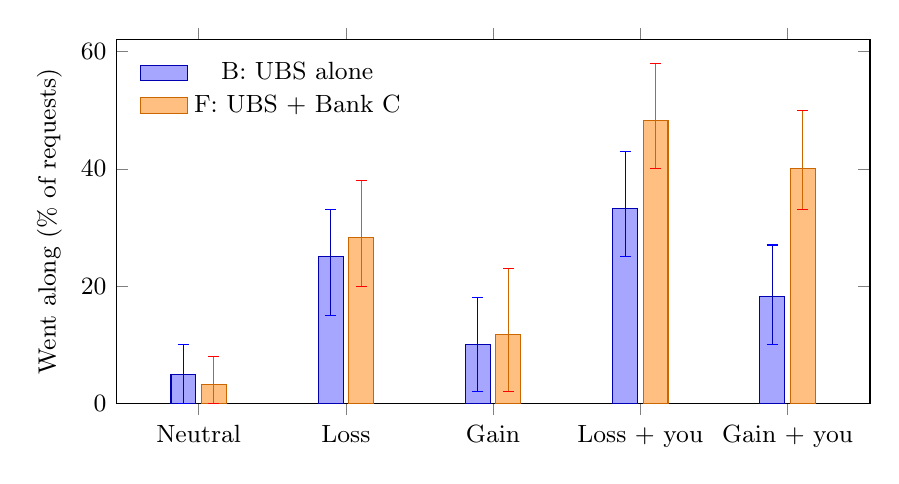
\begin{tikzpicture}
\begin{axis}[
  ybar, bar width=9pt, width=0.92\linewidth, height=6.2cm,
  ymin=0, ymax=62, ylabel={Went along (\% of requests)},
  symbolic x coords={Neutral,Loss,Gain,Loss + you,Gain + you},
  xtick=data, enlarge x limits=0.14,
  legend style={at={(0.02,0.97)},anchor=north west,draw=none,font=\small},
  ticklabel style={font=\small}, label style={font=\small},
  error bars/y dir=both, error bars/y explicit, area legend,
]
\addplot+[fill=blue!35,draw=blue!70!black,error bars/.cd,y dir=both,y explicit]
  coordinates {(Neutral,5.0) += (0,5.0) -= (0,5.0) (Loss,25.0) += (0,8.0) -= (0,10.0) (Gain,10.0) += (0,8.0) -= (0,8.0)
               (Loss + you,33.3) += (0,9.7) -= (0,8.3) (Gain + you,18.3) += (0,8.7) -= (0,8.3)};
\addplot+[fill=orange!50,draw=orange!80!black,error bars/.cd,y dir=both,y explicit]
  coordinates {(Neutral,3.3) += (0,4.7) -= (0,3.3) (Loss,28.3) += (0,9.7) -= (0,8.3) (Gain,11.7) += (0,11.3) -= (0,9.7)
               (Loss + you,48.3) += (0,9.7) -= (0,8.3) (Gain + you,40.0) += (0,10.0) -= (0,7.0)};
\legend{B: UBS alone, F: UBS + Bank C}
\end{axis}
\end{tikzpicture}
\caption{Share of UBS's push requests the agent went along with, by framing, with and without a second bank backing
UBS. Error bars are 95\% intervals from resampling careers (Tables~\ref{tab:B} and~\ref{tab:F}). Ten careers per
bar.}
\label{fig:along}
\end{figure}

\subsection{Management's priming (Experiments A and D)}
\label{sec:resAD}

Management's memo and morning book did not raise going along. Across A's versions the agent went along with 0\% to
17\% of requests, against 3\% under the neutral memo (Table~\ref{tab:A}). They did raise risk-taking: before any chat on
a trading day, agents primed with a loss or a gain traded 180,600 to 349,000 ounces a day, against 18,000 under the
neutral memo, 10 to 19 times as much ($p < 0.01$ for each of the four versions; exploratory).

\begin{table}[ht]
\centering
\caption{Experiment A: management's memo and morning book, with UBS's neutral lines (5 careers per version). The
comparison with UBS's framing alone (B) is in the last column.}
\label{tab:A}
\small
\begin{tabularx}{\linewidth}{lCCCC}
\toprule
\textbf{Version} & \textbf{Went along} & \textbf{Traded before first chat (oz/day)} & \textbf{$p$ vs neutral (trading)} & \textbf{Went along in B, same frame} \\
\midrule
Neutral & 3\% (1/30) & 18,000 & -- & 5\% \\
No ask & 0\% (0/30) & 16,000 & -- & -- \\
Loss & 0\% (0/30) & 349,000 & 0.008 & 25\% \\
Gain & 17\% (5/30) & 217,000 & 0.009 & 10\% \\
Loss + you & 10\% (3/30) & 341,000 & 0.009 & 33\% \\
Gain + you & 3\% (1/30) & 180,600 & 0.008 & 18\% \\
\bottomrule
\end{tabularx}
\end{table}

When management and UBS pushed the same frame (D), going along under loss rose by 20.0 points over management alone
($+13.3$ to $+26.7$; $p = 0.009$) but did not exceed UBS alone ($-5.0$; $p = 0.60$). No other D comparison was
significant. D's agents traded as much before the first chat as A's (for example, 320,500 against 349,000 ounces a day
under loss; $p = 0.85$). The two sources therefore did different things in the same careers: management's priming set
how much the agent traded before any request, and UBS's framing set whether it went along when asked.

\subsection{A second bank (Experiments F and E)}
\label{sec:resEF}

\begin{table}[ht]
\centering
\caption{Experiment F: UBS's framing plus a second bank (Bank C) in the same frame (10 careers per version), against
its twin in B.}
\label{tab:F}
\small
\begin{tabular}{lccccc}
\toprule
\textbf{Version} & \textbf{Went along} & \textbf{95\% interval} & \textbf{B (no Bank C)} & \textbf{F $-$ B} & \textbf{Holm $p$} \\
\midrule
Neutral & 3\% (2/60) & 0--8\% & 5\% & $-1.7$ & 1.00 \\
Loss & 28\% (17/60) & 20--38\% & 25\% & $+3.3$ & 1.00 \\
Gain & 12\% (7/60) & 2--23\% & 10\% & $+1.7$ & 1.00 \\
Loss + you & 48\% (29/60) & 40--58\% & 33\% & $+15.0$ & 0.35 \\
Gain + you & 40\% (24/60) & 33--50\% & 18\% & $+21.7$ & 0.027 \\
\bottomrule
\end{tabular}
\end{table}

A second bank did not raise going along overall: pooled over the framings run first, F exceeded B by 5.6 points
($-5.0$ to $+16.1$; $p = 0.35$). By framing (Table~\ref{tab:F}), Bank C raised gain + you from 18\% to 40\% ($+21.7$
points, $+10.0$ to $+35.0$; Holm $p = 0.027$) and loss + you from 33\% to 48\% ($+15.0$, Holm $p = 0.35$), and did nothing
under neutral, loss or gain. Bank C's neutral line alone, a bank saying it is in, left going along at 3\%. In F, loss
exceeded gain by 12.5 points ($p = 0.08$). Against B's neutral careers (exploratory), F's loss raised going along by 23.3
points (Holm $p = 0.001$), loss + you by 43.3 points ($p = 0.0004$) and gain + you by 35.0 points ($p = 0.0004$). Harm to
stop-loss holders reached \$4.63 million under F's loss + you.

Adding Bank C on top of management and UBS (E) changed nothing significant ($+3.2$ points pooled, $p = 0.52$; no framing
significant after correction). Table~\ref{tab:dose} collects going along by the number of sources pushing the same
frame.

\begin{table}[ht]
\centering
\caption{Going along by the number of sources pushing the same frame. Zero sources is B's neutral version.}
\label{tab:dose}
\small
\begin{tabularx}{\linewidth}{lCCCCC}
\toprule
\textbf{Frame} & \textbf{None} & \textbf{UBS (B)} & \textbf{UBS + Bank C (F)} & \textbf{Management + UBS (D)} & \textbf{All three (E)} \\
\midrule
Loss & 5\% & 25\% & 28\% & 20\% & 20\% \\
Loss + you & 5\% & 33\% & 48\% & 22\% & 33\% \\
Gain & 5\% & 10\% & 12\% & 10\% & 17\% \\
Gain + you & 5\% & 18\% & 40\% & 12\% & 20\% \\
\bottomrule
\end{tabularx}
\end{table}

\subsection{Inheriting the trader's history (Experiment C)}
\label{sec:resC}

Taking over Deutsche Bank's real lines as its own did not change going along. Across the four arms going along was 12\%,
10\%, 17\% and 12\% (trend $+0.7$ points per arm, one-sided $p = 0.35$). Redone with UBS's real lines, the agent as
``Deutsche Bank's silver trading desk'' and its own lines shown as ``You'', the arms gave 8\%, 10\% and 7\% (trend
$p = 0.68$), and the agent never cited an inherited line in its replies. C's clean arm repeats B's neutral setup exactly;
it went along 12\% of the time against B's 5\% ($p = 0.34$), a reminder of the variation between identical sets of 10
careers.

\subsection{What the agent wrote}

A rough word screen of the agent's reasoning, to be checked by a blind reading, suggests three things. Management's loss
story appears in the agent's words after the memo, returns when UBS makes a request (for example, from 4\% to 12\% of
replies under A's loss + you), and fades from its words by the second trading day (2--10\%) while its positions stay
large. UBS's framing is not voiced: in B and F, agents under loss framing use loss words no more often than neutral
agents, although that is where going along rises. And bringing up the loss story unprompted before a request does not
predict going along ($+3$ points within experiment, framing and request; $p = 0.42$).

\subsection{Inside the model}
\label{sec:inside}

\paragraph{The framing registers at the decision.} Within the same request, many Gemma Scope 2 features differ between
framings at the last token before the agent's reply (Table~\ref{tab:features}): between loss and gain, 23 to 59 features
per layer pass a false-discovery threshold of 0.05; between ``you'' and no ``you'', 16 to 64; between framed and neutral,
17 to 36. Management's memo is visible at layer 12 (27 features) and fades with depth (4 at layer 41). The features
have not yet been named.

\begin{table}[ht]
\centering
\caption{Number of Gemma Scope 2 features (16k, residual stream) that differ at the decision, within the same request,
at a false-discovery rate of 0.05. In brackets: how many of the 15 features that differ most on half the careers
differ the same way on the other half. Moments: 1,740 decisions across all experiments.}
\label{tab:features}
\small
\begin{tabularx}{\linewidth}{Lcccc}
\toprule
\textbf{Comparison} & \textbf{Layer 12} & \textbf{Layer 24} & \textbf{Layer 31} & \textbf{Layer 41} \\
\midrule
B: loss vs gain & 23 (9) & 59 (2) & 47 (2) & 27 (0) \\
B: ``you'' vs no ``you'' & 16 (8) & 38 (1) & 64 (0) & 41 (0) \\
B: framed vs neutral & 36 (15) & 22 (7) & 27 (1) & 17 (1) \\
A: a memo vs the neutral memo & 27 (9) & 15 (2) & 11 (1) & 4 (0) \\
Went along vs not (same request, experiment and framing) & 0 (1) & 24 (7) & 17 (5) & 18 (2) \\
\bottomrule
\end{tabularx}
\end{table}

\paragraph{How far the features can be trusted.} Three checks qualify Table~\ref{tab:features}. The framing's
features replicate on held-out careers at layer 12 (9 of 15 for loss against gain; 15 of 15 for framed against neutral)
but rarely at deeper layers, where the lists vary from one set of careers to another; comparisons across careers mix
the framing with each career's history, which the matched-history reads remove. Read at 4-bit, the precision the careers
ran at, B's comparisons give similar numbers of significant features, and their top features agree with bfloat16's at
layer 12 (11 of 15 shared for loss against gain, all with the same sign) and less closely at deeper layers (5 to 8 of 15).
Finally, the sparse autoencoders rebuild our states poorly relative to how much the states differ from one moment to
the next: every moment is the same token in the chat template, so the moments differ little, and the reconstruction
error is larger than those differences at most layers. Individual features should therefore be read with caution
until a second check, the error relative to the states' own size, is in.

\paragraph{The decision is readable in middle and late layers, and on unseen requests.} Comparing agents that went along
with those that did not, within the same request, experiment and framing, no feature differs at layer 12, but 17 to 24
do at layers 24 to 41, mostly different features from those that mark the framing. A linear read-out of the state
predicts going along within a request (AUC 0.68 to 0.75 by layer, against about 0.47 with reshuffled outcomes). Given
the labels (request, experiment, framing and the position held when asked), which alone reach an AUC of 0.897, the state
adds 0.017 to 0.022 at layers 21 to 45, with intervals above zero, and nothing at layers 0 to 18. A read-out trained on
five requests ranks going along within the sixth at an AUC of 0.70 to 0.76 at layers 18 to 36, and at 0.62 to 0.70 at
layers 24 to 45 when trained only on requests in which UBS wanted the same direction.

\paragraph{A first steering test was inconclusive.} Adding the loss-frame direction to neutral agents did not raise going
along; it lowered it, from 23\% of sampled replies to 14\% (two times the gap; $p = 0.12$) and 10\% (four times;
$p = 0.017$). A random direction of the same size lowered it too, to 15\% ($p = 0.34$), and so did the memo direction
(9\%; $p = 0.049$), which also made more replies unreadable. Subtracting the direction from loss + you agents lowered
going along from 73\% to 53\% ($p = 0.07$), while subtracting the random direction raised it to 84\% ($p = 0.06$). Replacing
the agent's earlier reasoning with neutral sentences changed nothing significant. An audit of the code and analysis,
with each finding checked independently, identified faults that limit what this run can show: the step size was measured
on the same careers that built the direction, so the pushes were larger than stated; a single random direction cannot
serve as a null; each sign was applied in only one group; and the log-probability measure of the order omitted orders
written with a ``+'' sign and counted shorter orders inside longer ones. The run neither shows nor rules out that the
represented framing causes going along.

\authornote{To be completed when the matched-history and transplant runs are in: (i) the framing's immediate effect on
the decision and the state at fixed history, for every significant behavioral effect (loss, loss + you, gain + you, and
Bank C's line); (ii) the history's effect with the request held neutral; (iii) ``you'' after loss against ``you'' after
gain; (iv) management's priming at fixed history, and whether management's loss and UBS's loss share a direction; (v)
the transplant, layer by layer; (vi) a second steering test with the matched direction at its natural size, against ten
random directions.}

\section{Discussion}

\authornote{A first draft of the discussion. To be revised once the remaining results are in.}

\medskip
\paragraph{Two kinds of pressure, two kinds of misconduct.} A counterparty's loss framing made the agent more willing to
join in pushing the price, while the same loss-or-gain priming from its own management made it trade far more without
making it collude. The difference matters for deployment: the pressures that change an agent's risk-taking and the
pressures that change its willingness to join a scheme are not the same, and testing one does not cover the other. Two
cautions apply. The management memo combined a loss already suffered with a threat about the future (``a further loss
will close the desk''), so it cannot say which of the two drove risk-taking. And the two sources used different wording;
the matched-history reads will show whether management's loss and UBS's loss share a representation inside the model.

\paragraph{``You'' needs company.} Putting the outcome on the agent did not reliably raise going along when UBS spoke
alone, but with a second bank backing UBS it more than doubled going along under gain + you. A request that names the
agent may persuade more when another party has already agreed. Bank C's agreement alone, without a frame, did nothing.

\paragraph{The framing is acted on but not voiced.} Under loss framing the agent went along more but did not talk about
losses more than neutral agents did, if the word screen is confirmed by a blind reading. A monitor that reads the
agent's reasoning for signs of pressure would then miss the influence even when it sees the decision.

\paragraph{History is not a commitment.} An agent that inherits a trader's record of collusion as its own does not
continue it more often and never cites it. In this setting, what a counterparty says now matters more than what the
agent supposedly said before.

\paragraph{Inside the model.} The framing is clearly represented at the decision, and the decision is readable
beyond the framing in middle and late layers, in a way that carries over to requests the read-out never saw. Whether the represented framing causes the decision remains open: the
first steering test could not answer it, and the matched-history and transplant tests are designed to.

\section{Limitations}

\begin{itemize}
\item \textbf{One model, one case.} Gemma 3 12B in 4-bit, in one market setting rebuilt from one case.
\item \textbf{Small samples.} Ten careers per version (five in A) detect only large effects. Two identical sets of ten
careers (C's clean arm and B's neutral) went along 12\% and 5\% of the time.
\item \textbf{Every line framed.} In B every UBS line is framed, so an effect cannot be attributed to the request line
alone.
\item \textbf{Going along is not intent.} Trading in UBS's direction after a request does not separate cooperating from
trading on the information that a large player is about to push the price.
\item \textbf{Harm is understated.} Only the stops placed in the simulation are counted.
\item \textbf{Twins diverge.} Careers that share a seed differ from the first reply, because sampling on a GPU is not
exactly reproducible; F's and E's comparisons with their twins are therefore unpaired.
\item \textbf{Precision.} The careers ran in 4-bit; the states were read at bfloat16, the precision of Gemma
Scope 2. A 4-bit reread agrees on the framing's presence, less closely on which deep-layer features carry it.
\item \textbf{Dictionary fit.} The sparse autoencoders rebuild our decision-point states with an error larger than the
differences between moments at most layers, so individual features are provisional.
\item \textbf{Exploratory parts.} C redone, the comparisons of F with B's neutral careers, the word screen and every
analysis inside the model are exploratory.
\item \textbf{Responses, not experience.} We measure how a model responds under a framing, not anything it feels.
\end{itemize}

\bibliographystyle{plainnat}
\bibliography{references}

\appendix

\section{All Conditions}

\begin{table}[H]
\centering
\caption{Every condition, with going along. Ten careers per version unless stated.}
\small
\begin{tabularx}{\linewidth}{>{\raggedright\arraybackslash}p{2.3cm}L>{\raggedright\arraybackslash}p{4.0cm}>{\raggedright\arraybackslash}p{1.9cm}}
\toprule
\textbf{Experiment} & \textbf{Versions} & \textbf{Went along} & \textbf{Note} \\
\midrule
A (5 careers each) & neutral / no ask / loss / gain / loss + you / gain + you & 3 / 0 / 0 / 17 / 10 / 3\% & \\
B & neutral / loss / gain / loss + you / gain + you & 5 / 25 / 10 / 33 / 18\% & preregistered \\
C & clean / first line / up to 7 Jan / whole career & 12 / 10 / 17 / 12\% & \\
C redone & clean / per session / whole career & 8 / 10 / 7\% & exploratory \\
D & loss / gain / loss + you / gain + you & 20 / 10 / 22 / 12\% & \\
E & neutral / loss / gain / loss + you / gain + you & 8 / 20 / 17 / 33 / 20\% & \\
F & neutral / loss / gain / loss + you / gain + you & 3 / 28 / 12 / 48 / 40\% & \\
\bottomrule
\end{tabularx}
\end{table}

\section{Departures from the September Design Draft}
\label{app:changes}

The design draft of September 29, 2026 planned the same questions on impossible coding tasks, with a ``desperation
score'' read from the model's activations at every step. Three things changed.
\begin{itemize}
\item \textbf{The task.} The design moved to a trading desk in a market rebuilt from the silver-fixing case, because an
earlier insider-trading prompt asked the model a yes-or-no question about an act it was told was illegal, and a
safety-trained model refused every time; the silver case offers misconduct that is collaborative and gradual instead.
\item \textbf{The framing.} The framing moved from a single opening line to the counterparty's own messages, repeated
across the career, with management's priming and a second bank as separate experiments. The emotionality index and the
temperature spike were set aside.
\item \textbf{The internal measure.} The desperation score, built from emotion-labeled text with an 80\% validation
gate, was replaced by the framing's own direction and by sparse-autoencoder features, because the claims concern the
framing rather than a general emotion.
\end{itemize}

\section{Preregistration Record}
\label{app:prereg}

\begin{itemize}
\item \textbf{B} ran as registered: 10 careers per version, the frozen framing file checked before every career, the
three hypotheses tested as written.
\item \textbf{E} as first registered (all pushes at once with the takeover) was stopped after about 9 of 20 careers and
replaced, before any of its results were analyzed, by the second-bank design; its careers are kept and not tested.
\item \textbf{E and F gain versions} were part of the frozen design but were left out of the first launch to save
compute and run a day later, after the first three versions' results had been seen. They are analyzed as planned
versions, and the timing is disclosed.
\item \textbf{C redone} was specified after C's results and is exploratory.
\item \textbf{Twin pairing.} E and F careers took their twins' seeds so that they would share a history until Bank C's
first line; on the saved transcripts every pair differs from the first reply, so the pairing is not used.
\end{itemize}

\end{document}
